\documentclass[11pt]{extarticle}
\usepackage{mathtools}
\usepackage[a4paper, total={6in, 8.5in}, top=1in, bottom=1in, left=1in, right=1in]{geometry}
\usepackage{graphicx}
\usepackage{subfig}
\usepackage{amssymb}
\usepackage{amsmath}
\usepackage{pythonhighlight}
\usepackage{pdfpages}
\usepackage[T1]{fontenc}
\usepackage[utf8]{inputenc}
\usepackage{fancyhdr}
\usepackage{pythonhighlight}
\usepackage{changepage}
\usepackage{slashbox}
\usepackage{floatrow}
\usepackage{subfig}
\usepackage{listings}
\usepackage[hidelinks]{hyperref}
\usepackage{fontawesome}
\usepackage{color} %red, green, blue, yellow, cyan, magenta, black, white
\definecolor{mygreen}{RGB}{28,172,0} % color values Red, Green, Blue
\definecolor{mylilas}{RGB}{170,55,241}


\floatsetup[table]{capposition=top}

\sloppy
\definecolor{lightgray}{gray}{0.5}
\setlength{\parindent}{0pt}
\setlength{\headheight}{14pt}

\renewcommand{\headrulewidth}{.4mm} % header line width
\newcommand{\norm}[1]{\left\lVert#1\right\rVert}




\pagestyle{fancy}
\fancyhf{}
\fancyhfoffset[L]{-1cm} % left extra length
\fancyhfoffset[R]{-1cm} % right extra length
\rhead{\bfseries Kutay U\u{g}urlu 2232841}
\lhead{EE583 Homework 4}
\rfoot{}

\DeclarePairedDelimiter\ceil{\lceil}{\rceil}
\DeclarePairedDelimiter\floor{\lfloor}{\rfloor}

\author{Kutay U\u{g}urlu 2232841}

\begin{document}

\lstset{language=Matlab,%
    %basicstyle=\color{red},
    breaklines=true,%
    morekeywords={matlab2tikz},
    keywordstyle=\color{blue},%
    morekeywords=[2]{1}, keywordstyle=[2]{\color{black}},
    identifierstyle=\color{black},%
    stringstyle=\color{mylilas},
    commentstyle=\color{mygreen},%
    showstringspaces=false,%without this there will be a symbol in the places where there is a space
    numbers=left,%
    numberstyle={\tiny \color{black}},% size of the numbers
    numbersep=9pt, % this defines how far the numbers are from the text
    emph=[1]{for,end,break},emphstyle=[1]\color{red}, %some words to emphasise
    %emph=[2]{word1,word2}, emphstyle=[2]{style},    
}

\fancyfoot[C]{\thepage}
\title{\LARGE \LARGE EE583 Pattern Recognition HW4}

\maketitle{\LARGE}

\pagebreak


\section{Question 1}

\begin{center}
    \begin{figure}[h]
        \begin{tabular}{cc}
            \subfloat[]{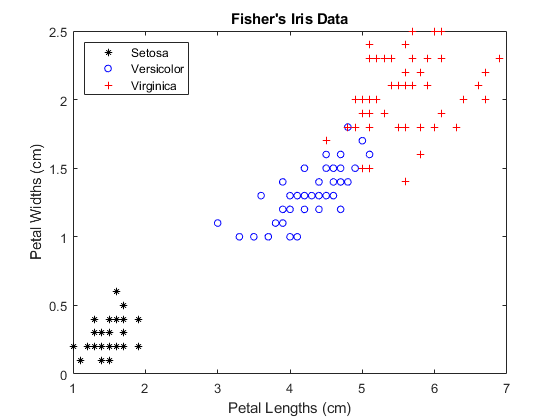
\includegraphics[width = 2in, height = 1.5in]{Q1_dist.png}} &
            \subfloat[]{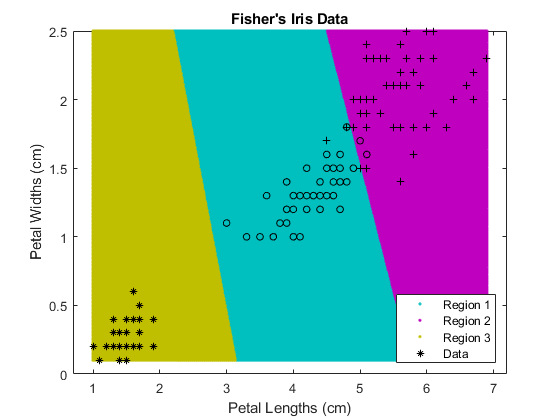
\includegraphics[width = 2in, height = 1.5in]{Q1_grid.png}}   \\
        \end{tabular}
        \caption{The data distribution and partitioning}
        \label{fig:q1fig}
    \end{figure}
\end{center}

\begin{center}
    \begin{figure}[h]
        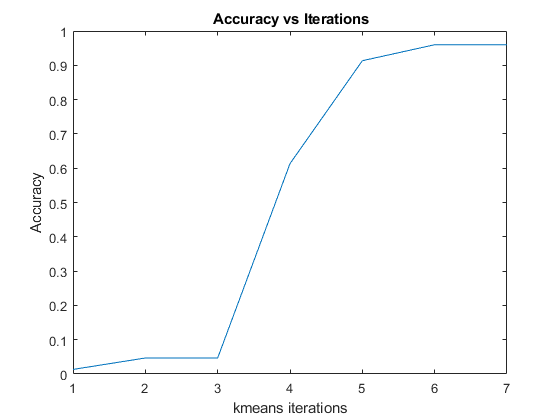
\includegraphics[width = 2in, height = 1.5in]{Q1_acc.png}
        \caption{classification success for different centroids}
        \label{fig:q1_2fig}
    \end{figure}
\end{center}

The centroids are manually set according to the approximate mean deduced from the data distribution plot. Initial centroids
can be found in \ref{subsec:Q1_code}. The accuracy is calculated in two steps. First, the confusion matrix is calculated, then the diagonal entries of it are added to obtain the true positive classifications. Finally, $Accuracy \triangleq \frac{\#TP}{\#Samples}$.
\\
Figure \ref{fig:q1_2fig} shows the accuracies of the iterations initialized with different centroids. Through careful centroid selection, the accuracy can be increased from 0.1 to 0.9647.

\pagebreak

\section{Question 2}

\begin{center}
    \begin{figure}[h]
        \begin{tabular}{cc}
            \subfloat[]{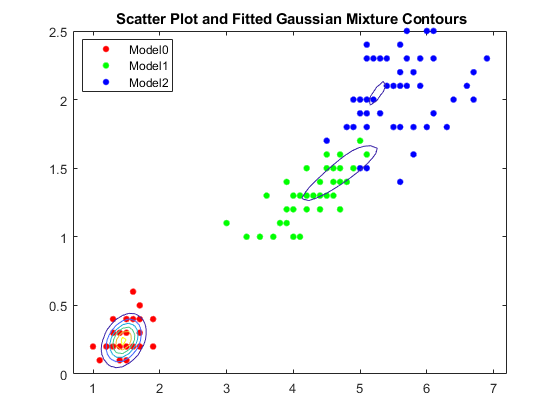
\includegraphics[width = 2in, height = 1.5in]{Q2.png}} &
            \subfloat[]{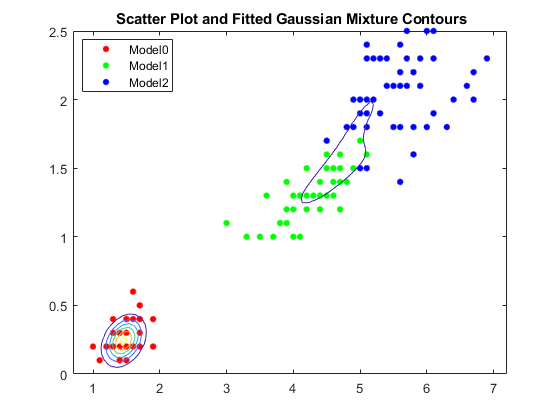
\includegraphics[width = 2in, height = 1.5in]{Q21.png}}  \\
        \end{tabular}
        \caption{The data distribution and partitioning}
        \label{fig:q2fig}
    \end{figure}
\end{center}



\section{Question 3}

\begin{center}
    \begin{figure}[h]
        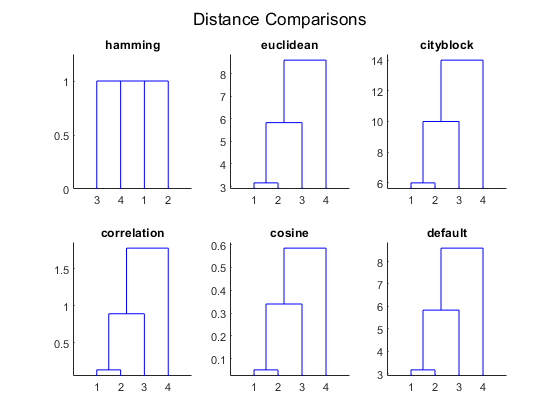
\includegraphics[width = 7in, height = 3in]{Q3.png}
        \caption{Dendrograms for different metrics}
        \label{fig:q3fig}
    \end{figure}
\end{center}


\pagebreak

\section{Question 4}

\subsection{Laplacian Matrix Normalization}
\begin{center}
    \begin{figure}[h]
        \begin{tabular}{cc}
            \subfloat[]{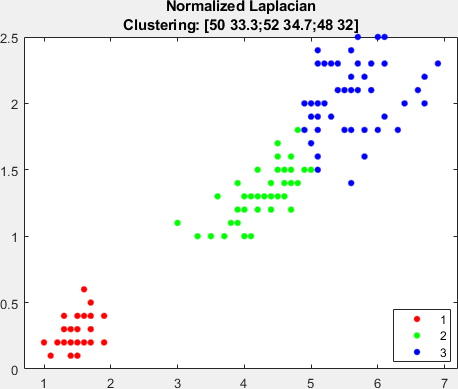
\includegraphics[width = 2in, height = 1.5in]{Q4_6.png}} &
            \subfloat[]{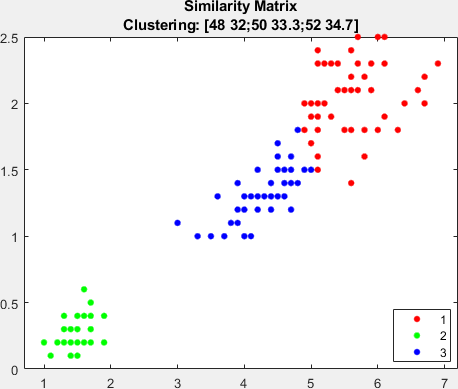
\includegraphics[width = 2in, height = 1.5in]{Q4_5.png}}   \\
        \end{tabular}
        \caption{Clustering for different cases}
        \label{fig:q41fig}
    \end{figure}
\end{center}
Using unnormalized Laplacian matrix increased the number of misclassifications.

\subsection{Distance Metrics}
\begin{center}
    \begin{figure}[h]
        \begin{tabular}{cc}
            \subfloat[]{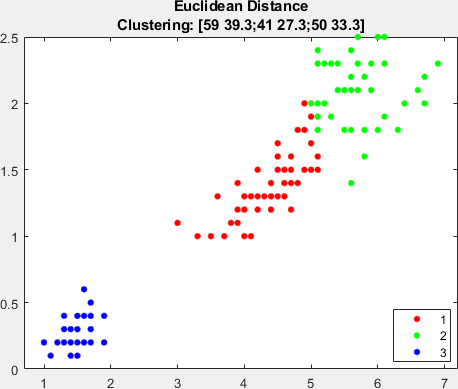
\includegraphics[width = 2in, height = 1.5in]{Q4_4.png}} &
            \subfloat[]{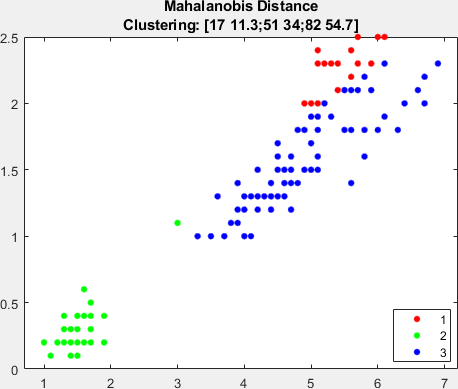
\includegraphics[width = 2in, height = 1.5in]{Q4_3.png}}   \\
        \end{tabular}
        \caption{Clustering for different cases}
        \label{fig:q42fig}
    \end{figure}
\end{center}

\subsection{Kernel Scale}
\begin{center}
    \begin{figure}[h]
        \begin{tabular}{cc}
            \subfloat[]{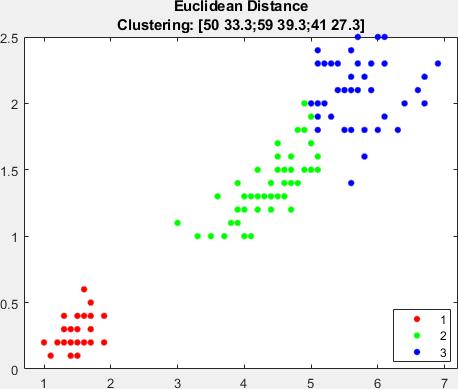
\includegraphics[width = 2in, height = 1.5in]{Q4_2.png}} &
            \subfloat[]{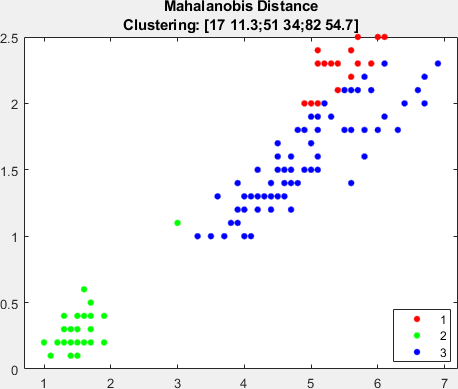
\includegraphics[width = 2in, height = 1.5in]{Q4_1.png}}   \\
        \end{tabular}
        \caption{Clustering for different cases}
        \label{fig:q43fig}
    \end{figure}
\end{center}

\pagebreak
\section{APPENDIX}
The code given in this section is shared \href{https://github.com/kutay-ugurlu/Pattern-Recognition/tree/master/HW4}{@\faGithubSquare}.
\subsection{Q1}\label{subsec:Q1_code}
\lstinputlisting{HW4_Q1.m}
\pagebreak
\subsection{Q2} \label{subsec:Q2_code}
\lstinputlisting{HW4_Q2.m}
\pagebreak
\subsection{Q3}\label{subsec:Q3_code}
\lstinputlisting{HW4_Q3.m}
\pagebreak
\subsection{Q4}\label{subsec:Q4_code}
\lstinputlisting{HW4_Q4.m}
\end{document}